%
% $RCSfile: data_transfer_object.tex,v $
%
% Copyright (C) 2002-2008. Christian Heller.
%
% Permission is granted to copy, distribute and/or modify this document
% under the terms of the GNU Free Documentation License, Version 1.1 or
% any later version published by the Free Software Foundation; with no
% Invariant Sections, with no Front-Cover Texts and with no Back-Cover
% Texts. A copy of the license is included in the section entitled
% "GNU Free Documentation License".
%
% http://www.cybop.net
% - Cybernetics Oriented Programming -
%
% http://www.resmedicinae.org
% - Information in Medicine -
%
% Version: $Revision: 1.1 $ $Date: 2008-08-19 20:41:06 $ $Author: christian $
% Authors: Christian Heller <christian.heller@tuxtax.de>
%

\subsubsection{Data Transfer Object}
\label{data_transfer_object_heading}
\index{Data Transfer Object Pattern}
\index{DTO}
\index{Assembler Object}
\index{Flat Data Structure}
\index{Translator Architecture}

\begin{figure}[ht]
    \begin{center}
       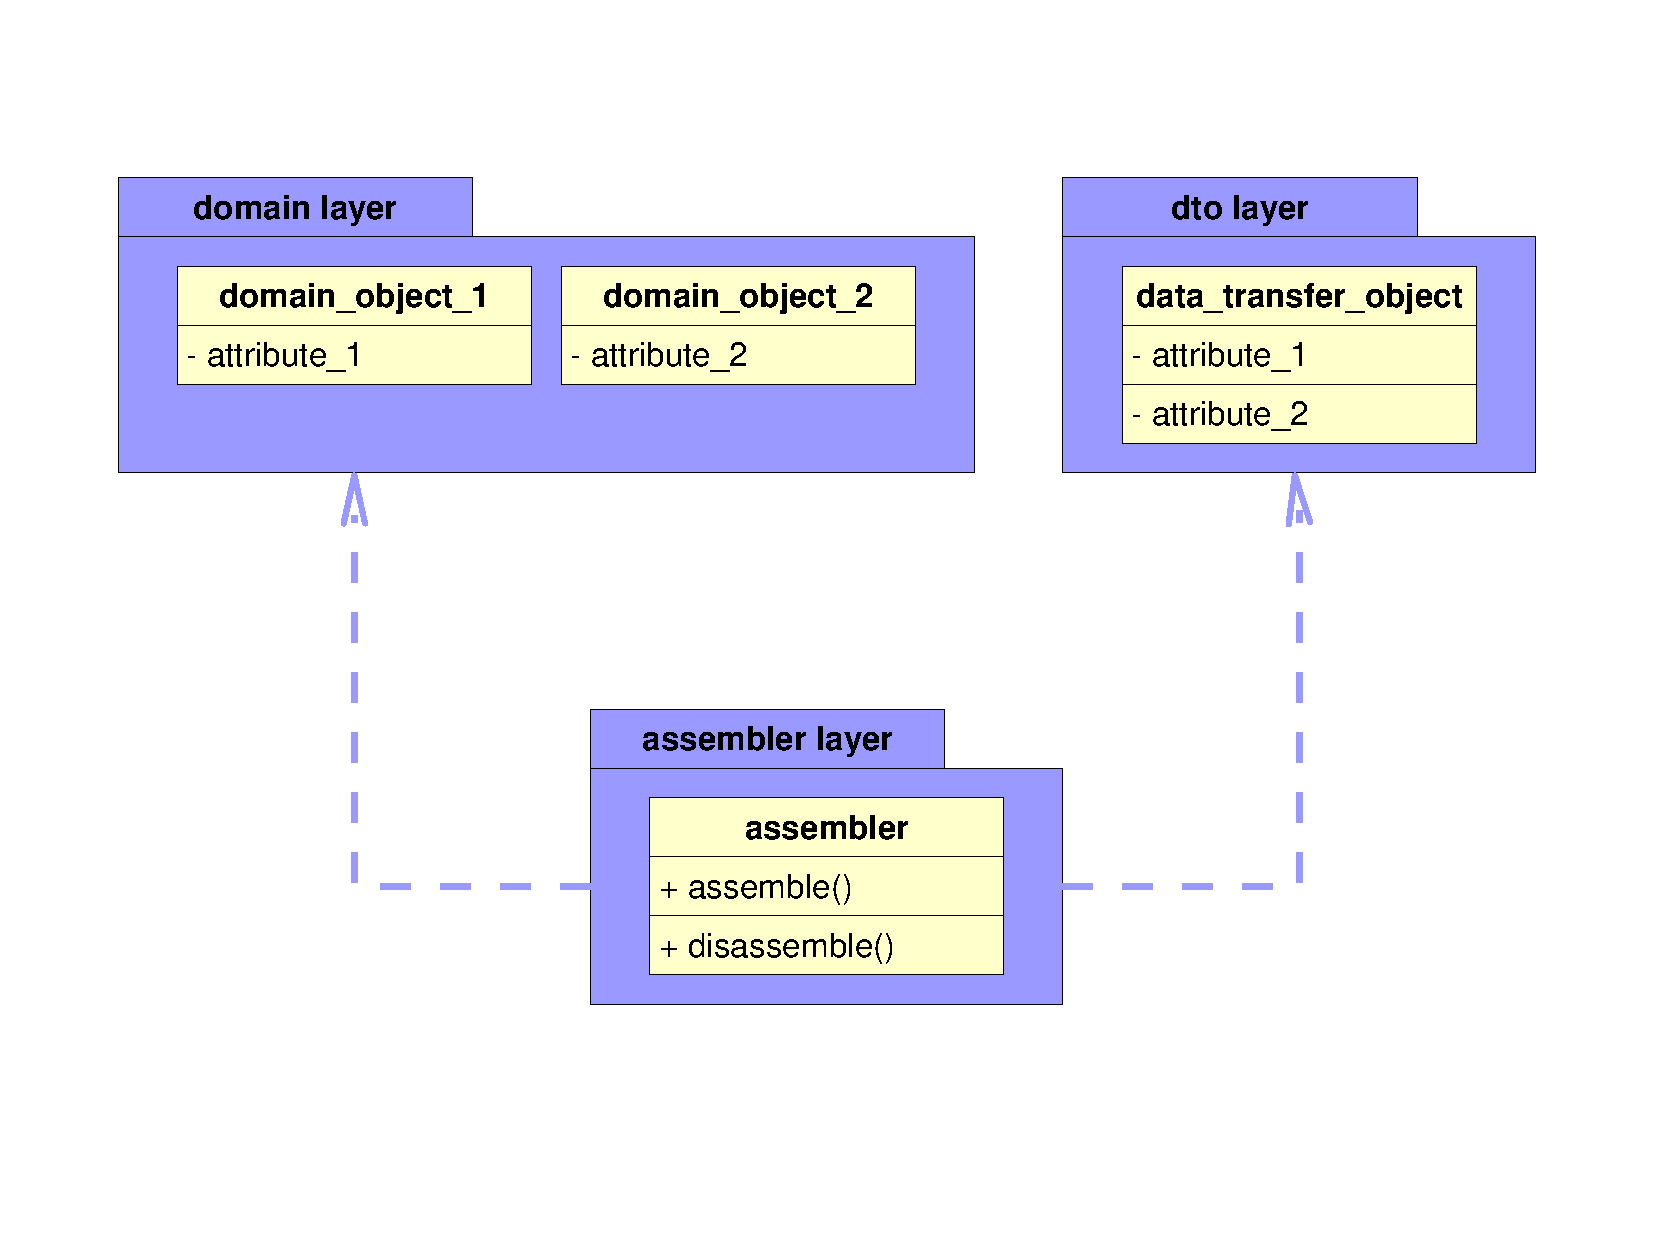
\includegraphics[scale=0.3,angle=-90]{graphic/dto.pdf}
       \caption{Data Transfer Object Pattern}
       \label{dto_figure}
    \end{center}
\end{figure}

It is a well-known fact that many small requests between two processes, and
even more between two hosts in a network need a lot of time. A local machine
with two processes has to permanently change the \emph{Program Context}; a
network has a lot of \emph{Transfers}. For each request, there is a necessity
of at least \emph{two} transfers -- the \emph{Question} of the client and the
\emph{Answer} of the server. Transfer methods are often expected to deliver
common data such as a Person's address, that is surname, first name, street,
zip-code, town and so on. These information is best retrieved by only
\emph{one} transfer call. That way, the client has to wait only once for a
server response and the server does not get too many single tasks. All address
data (in this example) would best be packaged together and sent back to the
client.

A scenario of that kind is exactly what the \emph{Data Transfer Object} pattern
\cite{fowler2002} proposes a solution for: A central \emph{Assembler} object
takes all common data of the server's domain model objects and assembles them
together into a special \emph{Data Transfer Object} (DTO), which is a flat data
structure (figure \ref{dto_figure}). The server will then send this DTO over
network to the client. On the client's side, a similar assembler takes the DTO,
finds out all received data and maps (disassembles) them to the client's domain
model. In that manner, a DTO is able to drastically improve the communication
performance.

Both, \emph{Data Mapper-} and DTO pattern translate one model into another. Due
to this similarity, chapter \ref{state_and_logic_heading} will try to merge
them into a common \emph{Translator} architecture.
